\section{Implementation}
The objective is to convert the raw data from the cameras into an image format suitable for the \gls{h265} encoder, specifically the \gls{p010} format.
The \gls{p010} format is a YCbCr 4:2:0 format with semi-interlaced data, where each channel has 10 bits per pixel stored in the most significant bits of 16-bit little-endian unsigned integers.

This transformation process can be divided into five parts: unpacking the raw bits from the camera, separating different polarization angles, performing debayering, converting to YCbCr color space, applying chroma subsampling, and finally arranging the data in the correct format.
The entire process is visualized in Figure \ref{fig:transform}.
By separating the angles of polarization, it becomes possible to analyze the polarization data after decompression.
This approach is inspired by the work of Vy Nguyen et al., where they sequentially separated the demosaicking of color and polarization data into two distinct steps \cite{nguyenTwoStepColorPolarizationDemosaicking2022}.

The goals it to turn the raw data from the \cams into an image format that can be passed to the \gls{h265} encoder, namely the \gls{p010} format, without losing information.
\gls{p010} is a YCbCr 4:2:0 format with with semi-interlaced data and 10 bits per channel stored in the most significant bits of 16 bit little-endian unsigned integers.

This transformation process can be divided into five distinct parts: unpacking the raw bits from the camera, separating different angles of polarization, performing debayering, translating the data to YCbCr color space, applying chroma subsampling, and packaging the data in the correct format.
The entire process is visually represented in Figure \ref{fig:transform}.
This approach is inspired by a research paper that introduced the concept of sequentially performing demosaicking of color and polarization data \cite{nguyenTwoStepColorPolarizationDemosaicking2022}.

\begin{figure}[H]
    \centering
    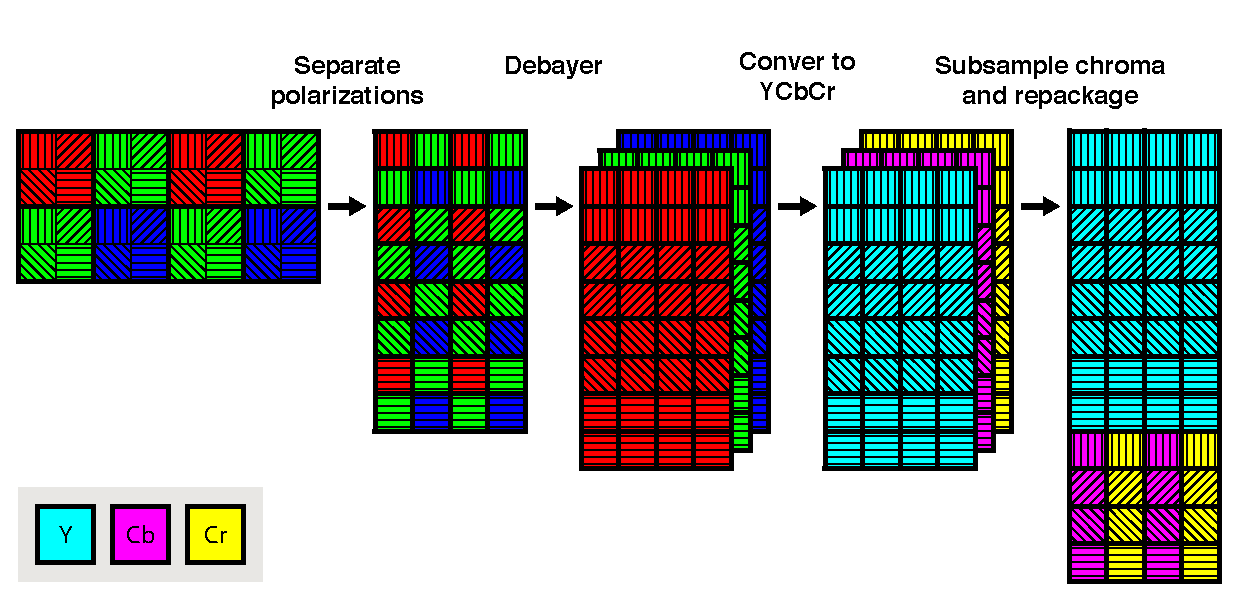
\includegraphics[width=\textwidth]{figures/polarized_image/transform.pdf}
    \caption{Visualization of how raw data is transforemd into a YCbCr format where the angles of polarization are stacked vertically.}
    \label{fig:transform}
\end{figure}

I initially tried performing these steps usind \gls{numpy} and \gls{opencv}.
But, even when levraging all eight \gls{cpu} cores to their full extent it was not possible to perform all the steps fast enough to keep up with the video input from both cameras.
Running the \gls{cpu} cores at max frequency also had a big inpact on the power consumption of the \jx.

In order to acheive the highest possible throughput, this whole transformation process formed in two steps and several performance optimizations are performed.










